%keep
\begin{figure*}[t]
\centering
\begin{subfigure}[b]{1.5in}
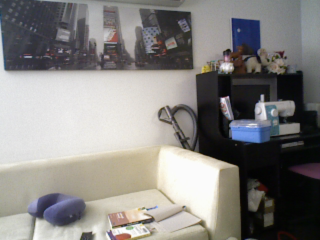
\includegraphics[width=1.5in]{{images/experiments/test_data/Apartment.Texture.rotate.0}.png}
\caption{Frame 1}
\end{subfigure}%
\begin{subfigure}[b]{1.5in}
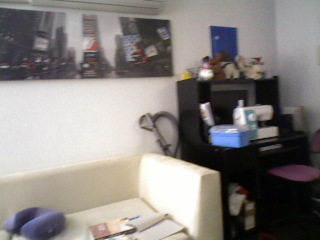
\includegraphics[width=1.5in]{{images/experiments/test_data/Apartment.Texture.rotate.1}.png}
\caption{Frame 10}
\end{subfigure}%
\begin{subfigure}[b]{1.5in}
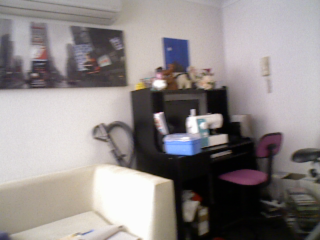
\includegraphics[width=1.5in]{{images/experiments/test_data/Apartment.Texture.rotate.2}.png}
\caption{Frame 15}
\end{subfigure}%
\begin{subfigure}[b]{1.5in}
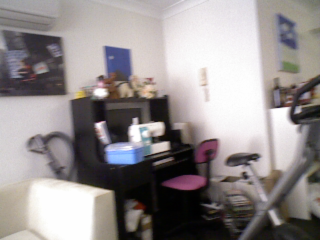
\includegraphics[width=1.5in]{{images/experiments/test_data/Apartment.Texture.rotate.3}.png}
\caption{Frame 20}
\end{subfigure}%
\caption{Four Sample Frames from the Apartment Texture Rotate Data Set}
\label{fig:Apartment_Texture_rotate}
\end{figure*}


%keep
\begin{figure*}[t]
\centering
\begin{subfigure}[b]{1.5in}
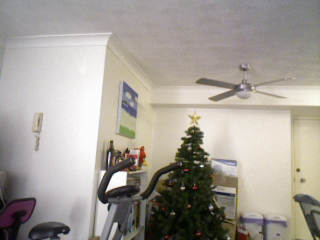
\includegraphics[width=1.5in]{{images/experiments/test_data/Apartment.Texture.rotateXAxis.0}.png}
\caption{Frame 1}
\end{subfigure}%
\begin{subfigure}[b]{1.5in}
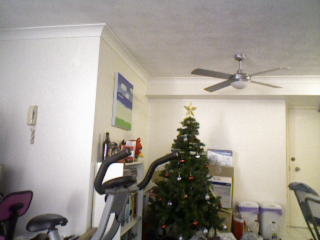
\includegraphics[width=1.5in]{{images/experiments/test_data/Apartment.Texture.rotateXAxis.1}.png}
\caption{Frame 10}
\end{subfigure}%
\begin{subfigure}[b]{1.5in}
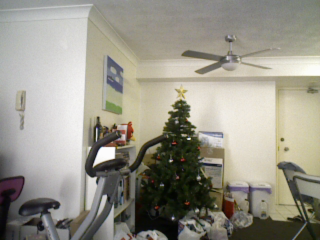
\includegraphics[width=1.5in]{{images/experiments/test_data/Apartment.Texture.rotateXAxis.2}.png}
\caption{Frame 15}
\end{subfigure}%
\begin{subfigure}[b]{1.5in}
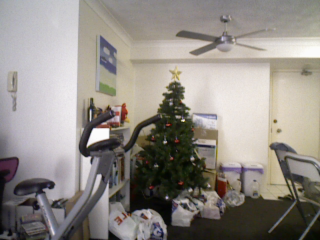
\includegraphics[width=1.5in]{{images/experiments/test_data/Apartment.Texture.rotateXAxis.3}.png}
\caption{Frame 20}
\end{subfigure}%
\caption{Four Sample Frames from the Apartment Texture X-Axis Rotation Data Set.}
\label{fig:Apartment_Texture_rotateXAxis}
\end{figure*}


%keep
\begin{figure*}[t]
\centering
\begin{subfigure}[b]{1.5in}
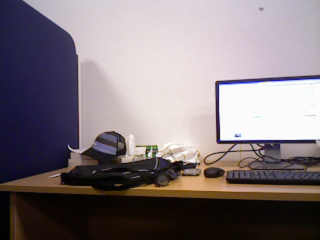
\includegraphics[width=1.5in]{{images/experiments/test_data/Desk.Texture.Translation.0}.png}
\caption{Frame 1}
\end{subfigure}%
\begin{subfigure}[b]{1.5in}
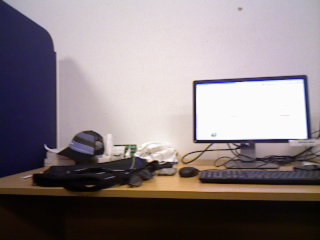
\includegraphics[width=1.5in]{{images/experiments/test_data/Desk.Texture.Translation.1}.png}
\caption{Frame 10}
\end{subfigure}%
\begin{subfigure}[b]{1.5in}
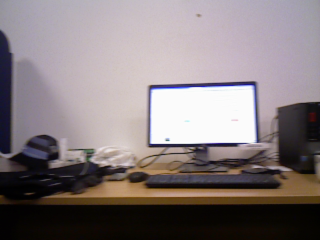
\includegraphics[width=1.5in]{{images/experiments/test_data/Desk.Texture.Translation.2}.png}
\caption{Frame 15}
\end{subfigure}%
\begin{subfigure}[b]{1.5in}
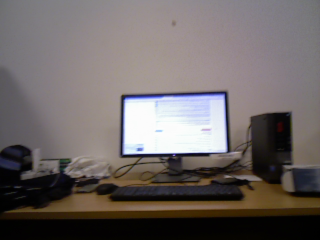
\includegraphics[width=1.5in]{{images/experiments/test_data/Desk.Texture.Translation.3}.png}
\caption{Frame 20}
\end{subfigure}%
\caption{Four Sample Frames from the Desk Texture Translation Data Set.}
\label{fig:Desk_Texture_Translation}
\end{figure*}


%keep
\begin{figure*}[t]
\centering
\begin{subfigure}[b]{1.5in}
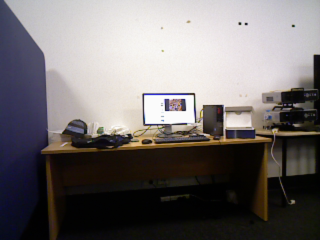
\includegraphics[width=1.5in]{{images/experiments/test_data/Office.Texture.blindSpotRotation.0}.png}
\caption{Frame 1}
\end{subfigure}%
\begin{subfigure}[b]{1.5in}
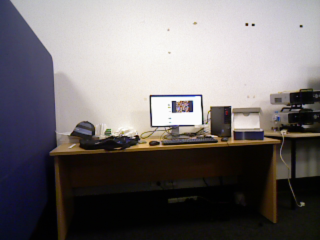
\includegraphics[width=1.5in]{{images/experiments/test_data/Office.Texture.blindSpotRotation.1}.png}
\caption{Frame 10}
\end{subfigure}%
\begin{subfigure}[b]{1.5in}
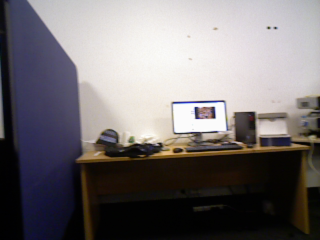
\includegraphics[width=1.5in]{{images/experiments/test_data/Office.Texture.blindSpotRotation.2}.png}
\caption{Frame 15}
\end{subfigure}%
\begin{subfigure}[b]{1.5in}
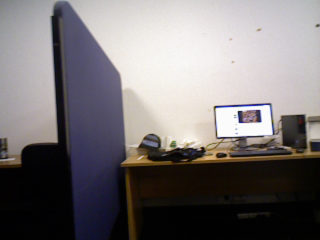
\includegraphics[width=1.5in]{{images/experiments/test_data/Office.Texture.blindSpotRotation.3}.png}
\caption{Frame 20}
\end{subfigure}%
\caption{Four Sample Frames from the Office Texture.blind-spot Rotation Data Set.}
\label{fig:Office_Texture_blindSpotRotation}
\end{figure*}


%keep
\begin{figure*}[t]
\centering
\begin{subfigure}[b]{1.5in}
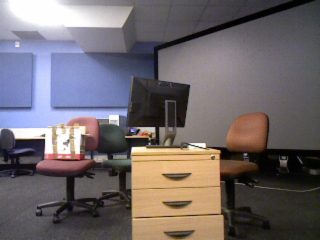
\includegraphics[width=1.5in]{{images/experiments/test_data/Office.TexturedItems.Translation.0}.png}
\caption{Frame 1}
\end{subfigure}%
\begin{subfigure}[b]{1.5in}
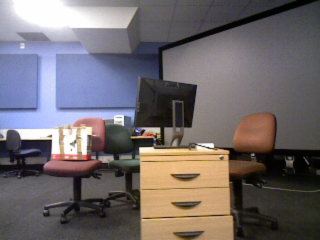
\includegraphics[width=1.5in]{{images/experiments/test_data/Office.TexturedItems.Translation.1}.png}
\caption{Frame 10}
\end{subfigure}%
\begin{subfigure}[b]{1.5in}
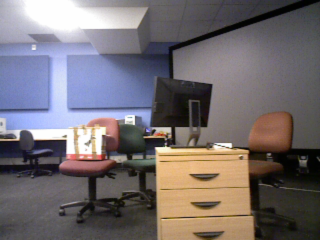
\includegraphics[width=1.5in]{{images/experiments/test_data/Office.TexturedItems.Translation.2}.png}
\caption{Frame 15}
\end{subfigure}%
\begin{subfigure}[b]{1.5in}
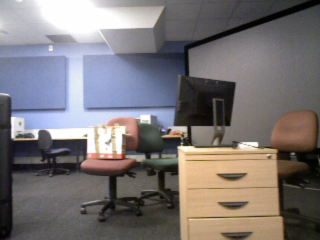
\includegraphics[width=1.5in]{{images/experiments/test_data/Office.TexturedItems.Translation.3}.png}
\caption{Frame 20}
\end{subfigure}%
\caption{Four Sample Frames from the Office Textured Items Translation Data Set.}
\label{fig:Office_TexturedItems_Translation}
\end{figure*}


%keep
\begin{figure*}[t]
\centering
\begin{subfigure}[b]{1.5in}
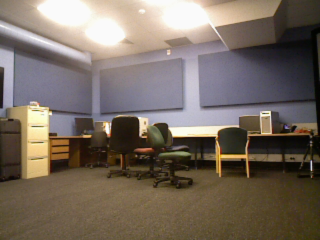
\includegraphics[width=1.5in]{{images/experiments/test_data/Office.Texture.rotation.0}.png}
\caption{Frame 1}
\end{subfigure}%
\begin{subfigure}[b]{1.5in}
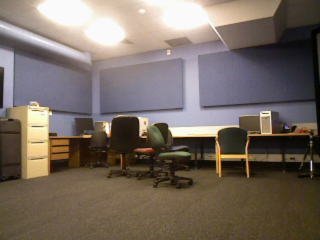
\includegraphics[width=1.5in]{{images/experiments/test_data/Office.Texture.rotation.1}.png}
\caption{Frame 10}
\end{subfigure}%
\begin{subfigure}[b]{1.5in}
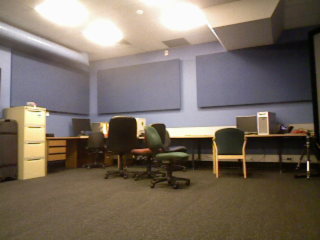
\includegraphics[width=1.5in]{{images/experiments/test_data/Office.Texture.rotation.2}.png}
\caption{Frame 15}
\end{subfigure}%
\begin{subfigure}[b]{1.5in}
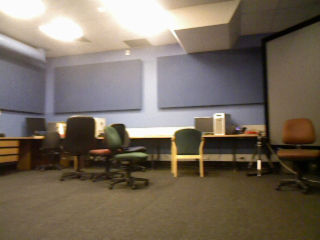
\includegraphics[width=1.5in]{{images/experiments/test_data/Office.Texture.rotation.3}.png}
\caption{Frame 20}
\end{subfigure}%
\caption{Four Sample Frames from the Office Texture Rotation Data Set.}
\label{fig:Office_Texture_rotation}
\end{figure*}

